
% This LaTeX was auto-generated from MATLAB code.
% To make changes, update the MATLAB code and republish this document.

\documentclass{article}
\usepackage{graphicx}
\usepackage{color}

\sloppy
\definecolor{lightgray}{gray}{0.5}
\setlength{\parindent}{0pt}

\begin{document}

    
    

\section*{2. Chebyshev points and interpolants}

\begin{verbatim}
ATAPformats
\end{verbatim}
\begin{par}
Any interval $[a,b]$ can be scaled to $[-1,1]$, so most of the time, we shall just talk about $[-1,1]$.
\end{par} \vspace{1em}
\begin{par}
Let $n$ be a positive integer:
\end{par} \vspace{1em}
\begin{par}
 \vspace{-2em} 
\end{par} \vspace{1em}
\begin{verbatim}
n = 16;
\end{verbatim}
\begin{par}
Consider $n+1$ equally spaced angles $\{\theta_j\}$ from 0 to $\pi$:
\end{par} \vspace{1em}
\begin{par}
 \vspace{-2em} 
\end{par} \vspace{1em}
\begin{verbatim}
tt = linspace(0,pi,n+1);
\end{verbatim}
\begin{par}
We can think of these as the arguments of $n+1$ points $\{z_j\}$ on the upper half of the unit circle in the complex plane.  These are the $(2n)\!\!$ th roots of unity lying in the closed upper half-plane:
\end{par} \vspace{1em}
\begin{par}
 \vspace{-2em} 
\end{par} \vspace{1em}
\begin{verbatim}
zz = exp(1i*tt);
hold off, plot(zz,'.-k'), axis equal, ylim([0 1.1])
FS = 'fontsize';
title('Equispaced points on the unit circle',FS,9)
\end{verbatim}

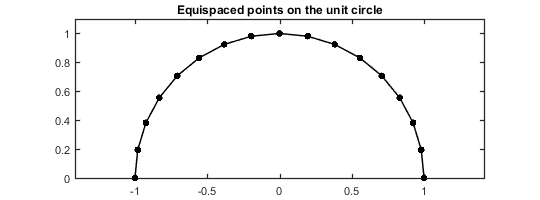
\includegraphics [width=4in]{chap2_01.png}
\begin{par}
 \vskip 1pt 
\end{par} \vspace{1em}
\begin{par}
The \textit{Chebyshev points} associated with the parameter $n$ are the real parts of these points,
\end{par} \vspace{1em}
\begin{par}
 \vskip -1.5em
$$ x_j = \hbox{Re}\, z_j = {1\over 2} (z_j^{} + z_j^{-1}),
\quad 0 \le j \le n: \eqno (2.1) $$
\vspace{-2em} 
\end{par} \vspace{1em}
\begin{verbatim}
xx = real(zz);
\end{verbatim}
\begin{par}
Some authors use the terms \textit{Chebyshev--Lobatto points}, \textit{Chebyshev extreme points}, or \textit{Chebyshev points of the second kind}, but as these are the points most often used in practical computation, we shall just say Chebyshev points.
\end{par} \vspace{1em}
\begin{par}
Another way to define the Chebyshev points is in terms of the original angles,
\end{par} \vspace{1em}
\begin{par}
 \vskip -2em
$$ x_j = \cos(\kern .7pt j \pi / n), \quad 0 \le j \le n, \eqno (2.2) $$
\vskip -1.5em 
\end{par} \vspace{1em}
\begin{verbatim}
xx = cos(tt);
\end{verbatim}
\begin{par}

\noindent
and the problem of polynomial interpolation in these points was
considered at least as early as [Jackson 1913]. There is also an
equivalent Chebfun command \verb|chebpts|:

\end{par} \vspace{1em}
\begin{par}
 \vspace{-2em} 
\end{par} \vspace{1em}
\begin{verbatim}
xx = chebpts(n+1);
\end{verbatim}
\begin{par}
Actually this result isn't exactly equivalent, as the ordering is left-to-right rather than right-to-left.  Concerning rounding errors when these numbers are calculated numerically, see Exercise 2.3.
\end{par} \vspace{1em}
\begin{par}
Let us add the Chebyshev points to the plot:
\end{par} \vspace{1em}
\begin{par}
 \vspace{-2em} 
\end{par} \vspace{1em}
\begin{verbatim}
hold on
for j = 2:n
  plot([xx(n+2-j) zz(j)],'k','linewidth',0.7)
end
plot(xx,0*xx,'.r'), title('Chebyshev points',FS,9)
\end{verbatim}

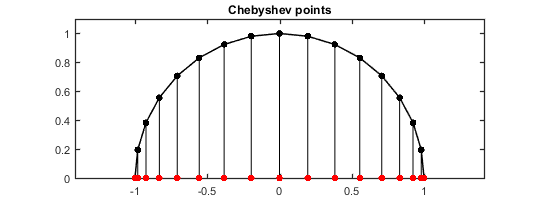
\includegraphics [width=4in]{chap2_02.png}
\begin{par}
 \vskip 1pt 
\end{par} \vspace{1em}
\begin{par}
They cluster near $1$ and $-1$, with the average spacing as $n\to\infty$ being given by a density function with square root singularities at both ends (Exercise 2.2).
\end{par} \vspace{1em}
\begin{par}

Let $\{f_j\}$, $0 \le j \le n$, be a set of numbers, which may or may not
come from sampling a function $f(x)$ at the Chebyshev points. Then there
exists a unique polynomial $p$ of degree $n$ that interpolates these
data, i.e., $p(x_j) = f_j$ for each~$j$.  When we say ``of degree $n$,''
we mean of degree less than or equal to $n$, and we let ${\cal P}_n$
denote the set of all such polynomials:
$$ {\cal P}_n = \{\hbox{polynomials of degree at most $n$}\}. \eqno (2.3) $$
As we trust the reader already knows, the existence and uniqueness of
polynomial interpolants applies for any distinct set of interpolation
points.  In the case of Chebyshev points, we call the polynomial the {\em
Chebyshev interpolant}.

\end{par} \vspace{1em}
\begin{par}
Polynomial interpolants through equally spaced points have terrible properties, as we shall see in Chapters 11--15. Polynomial interpolants through Chebyshev points, however, are excellent. It is the clustering near the ends of the interval that makes the difference, and other sets of points with similar clustering, like Legendre points (Chapter 17), have similarly good behavior.  The explanation of this fact has a lot to do with potential theory, a subject we shall introduce in Chapter 12. Specifically, what makes Chebyshev or Legendre points effective is that each one has approximately the same average distance from the others, as measured in the sense of the geometric mean.  On the interval $[-1,1]$, this distance is about $1/2$ (Exercise 2.6).
\end{par} \vspace{1em}
\begin{par}
Chebfun is built on Chebyshev interpolants [Battles \& Trefethen 2004]. For example, here is a certain step function:
\end{par} \vspace{1em}
\begin{par}
 \vskip -2em 
\end{par} \vspace{1em}
\begin{verbatim}
x = chebfun('x');
f = sign(x) - x/2;
hold off, plot(f,'k'), ylim([-1.3 1.3])
title('A step function',FS,9)
\end{verbatim}

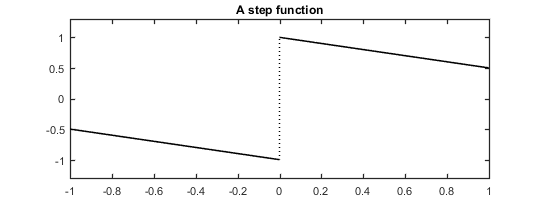
\includegraphics [width=4in]{chap2_03.png}
\begin{par}
 \vskip 1em
\noindent By calling \verb|chebfun| with a second explicit argument of 6,
we can construct the Chebyshev interpolant to $f$ through 6 points, that
is, of degree 5:

\end{par} \vspace{1em}
\begin{par}
 \vskip -2em 
\end{par} \vspace{1em}
\begin{verbatim}
p = chebfun(f,6); hold on, plot(p,'.-'), ylim([-1.3 1.3])
title('Degree 5 Chebyshev interpolant',FS,9)
\end{verbatim}

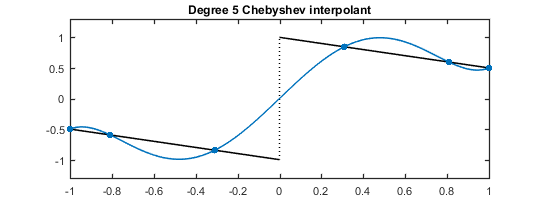
\includegraphics [width=4in]{chap2_04.png}
\begin{par}
 \vskip 1pt 
\end{par} \vspace{1em}
\begin{par}
Similarly, here is the Chebyshev interpolant of degree 25:
\end{par} \vspace{1em}
\begin{par}
 \vskip -2em 
\end{par} \vspace{1em}
\begin{verbatim}
hold off, plot(f,'k')
p = chebfun(f,26); hold on, plot(p,'.-')
ylim([-1.3 1.3]), title('Degree 25 Chebyshev interpolant',FS,9)
\end{verbatim}

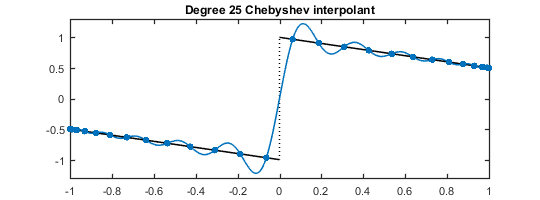
\includegraphics [width=4in]{chap2_05.png}
\begin{par}
 \vskip 1em
Here are a more complicated function and its interpolant of
degree 100:

\end{par} \vspace{1em}
\begin{par}
 \vskip -2em 
\end{par} \vspace{1em}
\begin{verbatim}
f = sin(6*x) + sign(sin(x+exp(2*x)));
hold off, plot(f,'k')
p = chebfun(f,101); hold on, plot(p), ylim([-2.4 2.4])
title('Degree 100 Chebyshev interpolant',FS,9)
\end{verbatim}

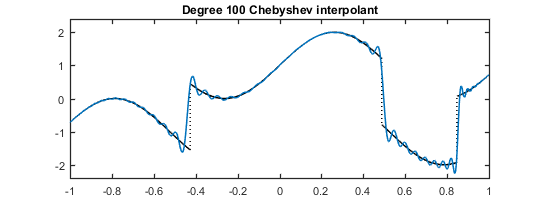
\includegraphics [width=4in]{chap2_06.png}
\begin{par}
 \vskip 1pt 
\end{par} \vspace{1em}
\begin{par}
Another way to use the \texttt{chebfun} command is by giving it an explicit vector of data rather than a function to sample, in which case it interprets the vector as data for a Chebyshev interpolant of the appropriate order.  Here for example is the interpolant of degree 99 through random data values at 100 Chebyshev points in $[-1,1]$:
\end{par} \vspace{1em}
\begin{par}
 \vskip -2em 
\end{par} \vspace{1em}
\begin{verbatim}
p = chebfun(2*rand(100,1)-1);
hold off, plot(p,'-'), hold on, plot(p,'.k')
ylim([-1.7 1.7]), grid on
title('Chebyshev interpolant through random data',FS,9)
\end{verbatim}

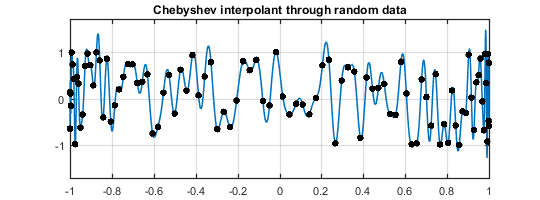
\includegraphics [width=4in]{chap2_07.png}
\begin{par}
 \vskip 1pt 
\end{par} \vspace{1em}
\begin{par}
This experiment illustrates how robust Chebyshev interpolation is.  If we had taken a million points instead of 100, the result would not have been much different mathematically, though it would have been a mess to plot. We shall return to this figure in Chapter 15.
\end{par} \vspace{1em}
\begin{par}
For illustrations like these it is interesting to pick data with jumps or wiggles, and Chapter 9 discusses such interpolants systematically.  In applications where polynomial interpolants are most useful, however, the data will typically be smooth.
\end{par} \vspace{1em}
\begin{par}

\begin{displaymath}
\framebox[4.7in][c]{\parbox{4.5in}{\vspace{2pt}\sl
{\sc Summary of Chapter 2.}
Polynomial interpolants in equispaced points in $[-1,1]$ have very poor
approximation properties, but interpolants in Chebyshev
points, which cluster near $\pm 1$, are excellent.\vspace{2pt}}}
\end{displaymath}

\end{par} \vspace{1em}
\begin{par}
 \smallskip\small\parskip=2pt
{\bf Exercise 2.1.  Chebyshev interpolants through random data.} (a)
Repeat the experiment of interpolation through random data for 10, 100,
1000, and 10000 points. In each case use {\tt minandmax(p)} to determine
the minimum and maximum values of the interpolant and measure the
computer time required for this computation $\hbox{(e.g.}$ using {\tt
tic} and {\tt toc}). You may find it helpful to increase Chebfun's
standard plotting resolution with a command like
\verb|plot(p,'numpts',10000)|. (b) In addition to the four plots over
$[-1,1]$, use {\tt plot(p,'.-','interval',[0.9999 1])} to produce another
plot of the 10000-point interpolant in the interval
$[0.9999,1]$. How many of the 10000 grid points fall in this interval?
\par
{\bf Exercise 2.2.  Limiting density as \boldmath$n\to\infty$.} (a)
Suppose $x_0,\dots,x_n$ are $n+1$ points equally spaced from $-1$ to $1$.
If $-1\le a < b \le 1$, what fraction of the points fall in the interval
$[a,b]$ in the limit $n\to\infty$?  Give an exact formula. (b) Give the
analogous formula for the case where $x_0,\dots ,x_n$ are the Chebyshev
points. (c) How does the result of (b) match the number found in
$[0.9999,1]$ in the last exercise for the case $n=9999$? (d) Show that
in the limit $n\to\infty$, the density of the Chebyshev points near $x\in
(-1,1)$ approaches $N/(\pi \sqrt{1-x^2}\kern 1pt)$ (see equation (12.10)).
\par
{\bf Exercise 2.3.  Rounding errors in computing Chebyshev points.} On a
computer in floating point arithmetic, the formula (2.2) for the
Chebyshev points is not so good, because it lacks the expected symmetries.
(a) Write a Matlab program that finds the smallest even value $n\ge 2$
for which, on your computer as computed by this formula, $x_{n/2} \ne 0$.
(You will probably find that $n=2$ is the first such value.)  (b) Find
the line in the code \verb|chebpts.m| in which Chebfun computes
Chebyshev points. What alternative formula does it use? Explain why this
formula achieves perfect symmetry for all $n$ in floating point
arithmetic. (c) Show that this formula is mathematically equivalent to
(2.2).
\par
{\bf Exercise 2.4. Chebyshev points of the first kind.} The Chebyshev
points of the first kind, also known as {\bf Gauss--Chebyshev points},
are obtained by taking the real parts of points on the unit circle
mid-way between those we have considered, i.e. $x_j = \cos( (\kern .7pt
j+{1\over 2}) \pi/(n+1))$ for integers $0\le j\le n$. Call {\tt help
chebpts} and {\tt help legpts} to find out how to generate these points
in Chebfun and how to generate Legendre points for comparison (these are
roots of Legendre polynomials---see Chapter 17).  For $n+1=100$, what
is the maximum difference between a Chebyshev point of the first kind and
the corresponding Legendre point?  Draw a plot to illustrate as
informatively as you can how close these two sets of points are.
\par
{\bf Exercise 2.5.  Convergence of Chebyshev interpolants.}  (a) Use
Chebfun to produce a plot on a log scale of $\|f-p_n\|$ as a function of
$n$ for $f(x) = e^x$ on $[-1,1]$, where $p_n$ is the Chebyshev
interpolant in ${\cal P}_n$.  Take $\|\cdot\|$ to be the supremum norm,
which can be computed by {\tt norm(f-p,inf)}.  How large must $n$ be for
accuracy at the level of machine precision?  What happens if $n$ is
increased beyond this point? (b) The same questions for $f(x) = 1/(1+25x^2)$.
Convergence rates like these will be analyzed in Chapters 7 and 8.
\par
{\bf Exercise 2.6.  Geometric mean distance between points.} Write a code
{\tt meandistance} that takes as input a vector of points $x_0,\dots,
x_n$ in $[-1,1]$ and produces a plot with $x_j$ on the horizontal axis
and the geometric mean of the distances of $x_j$ to the other points on the
vertical axis.  (The Matlab command {\tt prod} may be useful.) (a) What
are the results for Chebyshev points with $n = 5, 10, 20$? (b) The same for
Legendre points (see Exercise 2.4). (c) The same for equally spaced points
from $x_0=-1$ to $x_n = 1$.
\par
{\bf Exercise 2.7.  Chebyshev points scaled to the interval
\boldmath$[a,b]$.} (a) Use {\tt chebpts(10)} to print the values of the
Chebyshev points in $[-1,1]$ for $n=9$. (b) Use {\tt chebfun(@sin,10)} to
compute the degree 9 interpolant $p(x)$ to $\sin(x)$ in these points.
Make a plot showing $p(x)$ and $\sin(x)$ over the larger interval
$[-6,6]$, and also a semilog plot of $|f(x)-p(x)|$ over that interval.
Comment on the results. (c) Now use {\tt chebpts(10,[0 6])} to print the
values of the Chebyshev points for $n=9$ scaled to the interval $[0,6]$.
(d) Use {\tt chebfun(@sin,[0 6],10)} to compute the degree 9 interpolant
to $\sin(x)$ in these points, and make the same two plots as before over
$[-6,6]$.  Comment.
\par 
\end{par} \vspace{1em}



\end{document}
    
